% Options for packages loaded elsewhere
\PassOptionsToPackage{unicode}{hyperref}
\PassOptionsToPackage{hyphens}{url}
%
\documentclass[
]{article}
\usepackage{amsmath,amssymb}
\usepackage{iftex}
\ifPDFTeX
  \usepackage[T1]{fontenc}
  \usepackage[utf8]{inputenc}
  \usepackage{textcomp} % provide euro and other symbols
\else % if luatex or xetex
  \usepackage{unicode-math} % this also loads fontspec
  \defaultfontfeatures{Scale=MatchLowercase}
  \defaultfontfeatures[\rmfamily]{Ligatures=TeX,Scale=1}
\fi
\usepackage{lmodern}
\ifPDFTeX\else
  % xetex/luatex font selection
\fi
% Use upquote if available, for straight quotes in verbatim environments
\IfFileExists{upquote.sty}{\usepackage{upquote}}{}
\IfFileExists{microtype.sty}{% use microtype if available
  \usepackage[]{microtype}
  \UseMicrotypeSet[protrusion]{basicmath} % disable protrusion for tt fonts
}{}
\makeatletter
\@ifundefined{KOMAClassName}{% if non-KOMA class
  \IfFileExists{parskip.sty}{%
    \usepackage{parskip}
  }{% else
    \setlength{\parindent}{0pt}
    \setlength{\parskip}{6pt plus 2pt minus 1pt}}
}{% if KOMA class
  \KOMAoptions{parskip=half}}
\makeatother
\usepackage{xcolor}
\usepackage[margin=1in]{geometry}
\usepackage{graphicx}
\makeatletter
\def\maxwidth{\ifdim\Gin@nat@width>\linewidth\linewidth\else\Gin@nat@width\fi}
\def\maxheight{\ifdim\Gin@nat@height>\textheight\textheight\else\Gin@nat@height\fi}
\makeatother
% Scale images if necessary, so that they will not overflow the page
% margins by default, and it is still possible to overwrite the defaults
% using explicit options in \includegraphics[width, height, ...]{}
\setkeys{Gin}{width=\maxwidth,height=\maxheight,keepaspectratio}
% Set default figure placement to htbp
\makeatletter
\def\fps@figure{htbp}
\makeatother
\setlength{\emergencystretch}{3em} % prevent overfull lines
\providecommand{\tightlist}{%
  \setlength{\itemsep}{0pt}\setlength{\parskip}{0pt}}
\setcounter{secnumdepth}{-\maxdimen} % remove section numbering
<!--radix_placeholder_navigation_in_header-->
<meta name="distill:offset" content=""/>

<script type="application/javascript">

  window.headroom_prevent_pin = false;

  window.document.addEventListener("DOMContentLoaded", function (event) {

    // initialize headroom for banner
    var header = $('header').get(0);
    var headerHeight = header.offsetHeight;
    var headroom = new Headroom(header, {
      tolerance: 5,
      onPin : function() {
        if (window.headroom_prevent_pin) {
          window.headroom_prevent_pin = false;
          headroom.unpin();
        }
      }
    });
    headroom.init();
    if(window.location.hash)
      headroom.unpin();
    $(header).addClass('headroom--transition');

    // offset scroll location for banner on hash change
    // (see: https://github.com/WickyNilliams/headroom.js/issues/38)
    window.addEventListener("hashchange", function(event) {
      window.scrollTo(0, window.pageYOffset - (headerHeight + 25));
    });

    // responsive menu
    $('.distill-site-header').each(function(i, val) {
      var topnav = $(this);
      var toggle = topnav.find('.nav-toggle');
      toggle.on('click', function() {
        topnav.toggleClass('responsive');
      });
    });

    // nav dropdowns
    $('.nav-dropbtn').click(function(e) {
      $(this).next('.nav-dropdown-content').toggleClass('nav-dropdown-active');
      $(this).parent().siblings('.nav-dropdown')
         .children('.nav-dropdown-content').removeClass('nav-dropdown-active');
    });
    $("body").click(function(e){
      $('.nav-dropdown-content').removeClass('nav-dropdown-active');
    });
    $(".nav-dropdown").click(function(e){
      e.stopPropagation();
    });
  });
</script>

<style type="text/css">

/* Theme (user-documented overrideables for nav appearance) */

.distill-site-nav {
  color: rgba(255, 255, 255, 0.8);
  background-color: #0F2E3D;
  font-size: 15px;
  font-weight: 300;
}

.distill-site-nav a {
  color: inherit;
  text-decoration: none;
}

.distill-site-nav a:hover {
  color: white;
}

@media print {
  .distill-site-nav {
    display: none;
  }
}

.distill-site-header {

}

.distill-site-footer {

}


/* Site Header */

.distill-site-header {
  width: 100%;
  box-sizing: border-box;
  z-index: 3;
}

.distill-site-header .nav-left {
  display: inline-block;
  margin-left: 8px;
}

@media screen and (max-width: 768px) {
  .distill-site-header .nav-left {
    margin-left: 0;
  }
}


.distill-site-header .nav-right {
  float: right;
  margin-right: 8px;
}

.distill-site-header a,
.distill-site-header .title {
  display: inline-block;
  text-align: center;
  padding: 14px 10px 14px 10px;
}

.distill-site-header .title {
  font-size: 18px;
  min-width: 150px;
}

.distill-site-header .logo {
  padding: 0;
}

.distill-site-header .logo img {
  display: none;
  max-height: 20px;
  width: auto;
  margin-bottom: -4px;
}

.distill-site-header .nav-image img {
  max-height: 18px;
  width: auto;
  display: inline-block;
  margin-bottom: -3px;
}



@media screen and (min-width: 1000px) {
  .distill-site-header .logo img {
    display: inline-block;
  }
  .distill-site-header .nav-left {
    margin-left: 20px;
  }
  .distill-site-header .nav-right {
    margin-right: 20px;
  }
  .distill-site-header .title {
    padding-left: 12px;
  }
}


.distill-site-header .nav-toggle {
  display: none;
}

.nav-dropdown {
  display: inline-block;
  position: relative;
}

.nav-dropdown .nav-dropbtn {
  border: none;
  outline: none;
  color: rgba(255, 255, 255, 0.8);
  padding: 16px 10px;
  background-color: transparent;
  font-family: inherit;
  font-size: inherit;
  font-weight: inherit;
  margin: 0;
  margin-top: 1px;
  z-index: 2;
}

.nav-dropdown-content {
  display: none;
  position: absolute;
  background-color: white;
  min-width: 200px;
  border: 1px solid rgba(0,0,0,0.15);
  border-radius: 4px;
  box-shadow: 0px 8px 16px 0px rgba(0,0,0,0.1);
  z-index: 1;
  margin-top: 2px;
  white-space: nowrap;
  padding-top: 4px;
  padding-bottom: 4px;
}

.nav-dropdown-content hr {
  margin-top: 4px;
  margin-bottom: 4px;
  border: none;
  border-bottom: 1px solid rgba(0, 0, 0, 0.1);
}

.nav-dropdown-active {
  display: block;
}

.nav-dropdown-content a, .nav-dropdown-content .nav-dropdown-header {
  color: black;
  padding: 6px 24px;
  text-decoration: none;
  display: block;
  text-align: left;
}

.nav-dropdown-content .nav-dropdown-header {
  display: block;
  padding: 5px 24px;
  padding-bottom: 0;
  text-transform: uppercase;
  font-size: 14px;
  color: #999999;
  white-space: nowrap;
}

.nav-dropdown:hover .nav-dropbtn {
  color: white;
}

.nav-dropdown-content a:hover {
  background-color: #ddd;
  color: black;
}

.nav-right .nav-dropdown-content {
  margin-left: -45%;
  right: 0;
}

@media screen and (max-width: 768px) {
  .distill-site-header a, .distill-site-header .nav-dropdown  {display: none;}
  .distill-site-header a.nav-toggle {
    float: right;
    display: block;
  }
  .distill-site-header .title {
    margin-left: 0;
  }
  .distill-site-header .nav-right {
    margin-right: 0;
  }
  .distill-site-header {
    overflow: hidden;
  }
  .nav-right .nav-dropdown-content {
    margin-left: 0;
  }
}


@media screen and (max-width: 768px) {
  .distill-site-header.responsive {position: relative; min-height: 500px; }
  .distill-site-header.responsive a.nav-toggle {
    position: absolute;
    right: 0;
    top: 0;
  }
  .distill-site-header.responsive a,
  .distill-site-header.responsive .nav-dropdown {
    display: block;
    text-align: left;
  }
  .distill-site-header.responsive .nav-left,
  .distill-site-header.responsive .nav-right {
    width: 100%;
  }
  .distill-site-header.responsive .nav-dropdown {float: none;}
  .distill-site-header.responsive .nav-dropdown-content {position: relative;}
  .distill-site-header.responsive .nav-dropdown .nav-dropbtn {
    display: block;
    width: 100%;
    text-align: left;
  }
}

/* Site Footer */

.distill-site-footer {
  width: 100%;
  overflow: hidden;
  box-sizing: border-box;
  z-index: 3;
  margin-top: 30px;
  padding-top: 30px;
  padding-bottom: 30px;
  text-align: center;
}

/* Headroom */

d-title {
  padding-top: 6rem;
}

@media print {
  d-title {
    padding-top: 4rem;
  }
}

.headroom {
  z-index: 1000;
  position: fixed;
  top: 0;
  left: 0;
  right: 0;
}

.headroom--transition {
  transition: all .4s ease-in-out;
}

.headroom--unpinned {
  top: -100px;
}

.headroom--pinned {
  top: 0;
}

/* adjust viewport for navbar height */
/* helps vertically center bootstrap (non-distill) content */
.min-vh-100 {
  min-height: calc(100vh - 100px) !important;
}

</style>

<script src="site_libs/jquery-3.6.0/jquery-3.6.0.min.js"></script>
<link href="site_libs/font-awesome-6.4.2/css/all.min.css" rel="stylesheet"/>
<link href="site_libs/font-awesome-6.4.2/css/v4-shims.min.css" rel="stylesheet"/>
<script src="site_libs/headroom-0.9.4/headroom.min.js"></script>
<script src="site_libs/autocomplete-0.37.1/autocomplete.min.js"></script>
<script src="site_libs/fuse-6.4.1/fuse.min.js"></script>

<script type="application/javascript">

function getMeta(metaName) {
  var metas = document.getElementsByTagName('meta');
  for (let i = 0; i < metas.length; i++) {
    if (metas[i].getAttribute('name') === metaName) {
      return metas[i].getAttribute('content');
    }
  }
  return '';
}

function offsetURL(url) {
  var offset = getMeta('distill:offset');
  return offset ? offset + '/' + url : url;
}

function createFuseIndex() {

  // create fuse index
  var options = {
    keys: [
      { name: 'title', weight: 20 },
      { name: 'categories', weight: 15 },
      { name: 'description', weight: 10 },
      { name: 'contents', weight: 5 },
    ],
    ignoreLocation: true,
    threshold: 0
  };
  var fuse = new window.Fuse([], options);

  // fetch the main search.json
  return fetch(offsetURL('search.json'))
    .then(function(response) {
      if (response.status == 200) {
        return response.json().then(function(json) {
          // index main articles
          json.articles.forEach(function(article) {
            fuse.add(article);
          });
          // download collections and index their articles
          return Promise.all(json.collections.map(function(collection) {
            return fetch(offsetURL(collection)).then(function(response) {
              if (response.status === 200) {
                return response.json().then(function(articles) {
                  articles.forEach(function(article) {
                    fuse.add(article);
                  });
                })
              } else {
                return Promise.reject(
                  new Error('Unexpected status from search index request: ' +
                            response.status)
                );
              }
            });
          })).then(function() {
            return fuse;
          });
        });

      } else {
        return Promise.reject(
          new Error('Unexpected status from search index request: ' +
                      response.status)
        );
      }
    });
}

window.document.addEventListener("DOMContentLoaded", function (event) {

  // get search element (bail if we don't have one)
  var searchEl = window.document.getElementById('distill-search');
  if (!searchEl)
    return;

  createFuseIndex()
    .then(function(fuse) {

      // make search box visible
      searchEl.classList.remove('hidden');

      // initialize autocomplete
      var options = {
        autoselect: true,
        hint: false,
        minLength: 2,
      };
      window.autocomplete(searchEl, options, [{
        source: function(query, callback) {
          const searchOptions = {
            isCaseSensitive: false,
            shouldSort: true,
            minMatchCharLength: 2,
            limit: 10,
          };
          var results = fuse.search(query, searchOptions);
          callback(results
            .map(function(result) { return result.item; })
          );
        },
        templates: {
          suggestion: function(suggestion) {
            var img = suggestion.preview && Object.keys(suggestion.preview).length > 0
              ? `<img src="${offsetURL(suggestion.preview)}"</img>`
              : '';
            var html = `
              <div class="search-item">
                <h3>${suggestion.title}</h3>
                <div class="search-item-description">
                  ${suggestion.description || ''}
                </div>
                <div class="search-item-preview">
                  ${img}
                </div>
              </div>
            `;
            return html;
          }
        }
      }]).on('autocomplete:selected', function(event, suggestion) {
        window.location.href = offsetURL(suggestion.path);
      });
      // remove inline display style on autocompleter (we want to
      // manage responsive display via css)
      $('.algolia-autocomplete').css("display", "");
    })
    .catch(function(error) {
      console.log(error);
    });

});

</script>

<style type="text/css">

.nav-search {
  font-size: x-small;
}

/* Algolioa Autocomplete */

.algolia-autocomplete {
  display: inline-block;
  margin-left: 10px;
  vertical-align: sub;
  background-color: white;
  color: black;
  padding: 6px;
  padding-top: 8px;
  padding-bottom: 0;
  border-radius: 6px;
  border: 1px #0F2E3D solid;
  width: 180px;
}


@media screen and (max-width: 768px) {
  .distill-site-nav .algolia-autocomplete {
    display: none;
    visibility: hidden;
  }
  .distill-site-nav.responsive .algolia-autocomplete {
    display: inline-block;
    visibility: visible;
  }
  .distill-site-nav.responsive .algolia-autocomplete .aa-dropdown-menu {
    margin-left: 0;
    width: 400px;
    max-height: 400px;
  }
}

.algolia-autocomplete .aa-input, .algolia-autocomplete .aa-hint {
  width: 90%;
  outline: none;
  border: none;
}

.algolia-autocomplete .aa-hint {
  color: #999;
}
.algolia-autocomplete .aa-dropdown-menu {
  width: 550px;
  max-height: 70vh;
  overflow-x: visible;
  overflow-y: scroll;
  padding: 5px;
  margin-top: 3px;
  margin-left: -150px;
  background-color: #fff;
  border-radius: 5px;
  border: 1px solid #999;
  border-top: none;
}

.algolia-autocomplete .aa-dropdown-menu .aa-suggestion {
  cursor: pointer;
  padding: 5px 4px;
  border-bottom: 1px solid #eee;
}

.algolia-autocomplete .aa-dropdown-menu .aa-suggestion:last-of-type {
  border-bottom: none;
  margin-bottom: 2px;
}

.algolia-autocomplete .aa-dropdown-menu .aa-suggestion .search-item {
  overflow: hidden;
  font-size: 0.8em;
  line-height: 1.4em;
}

.algolia-autocomplete .aa-dropdown-menu .aa-suggestion .search-item h3 {
  font-size: 1rem;
  margin-block-start: 0;
  margin-block-end: 5px;
}

.algolia-autocomplete .aa-dropdown-menu .aa-suggestion .search-item-description {
  display: inline-block;
  overflow: hidden;
  height: 2.8em;
  width: 80%;
  margin-right: 4%;
}

.algolia-autocomplete .aa-dropdown-menu .aa-suggestion .search-item-preview {
  display: inline-block;
  width: 15%;
}

.algolia-autocomplete .aa-dropdown-menu .aa-suggestion .search-item-preview img {
  height: 3em;
  width: auto;
  display: none;
}

.algolia-autocomplete .aa-dropdown-menu .aa-suggestion .search-item-preview img[src] {
  display: initial;
}

.algolia-autocomplete .aa-dropdown-menu .aa-suggestion.aa-cursor {
  background-color: #eee;
}
.algolia-autocomplete .aa-dropdown-menu .aa-suggestion em {
  font-weight: bold;
  font-style: normal;
}

</style>


<!--/radix_placeholder_navigation_in_header-->
<!--radix_placeholder_site_in_header-->
<script type="text/javascript" cookie-consent="tracking" async src="https://www.googletagmanager.com/gtag/js?id=UA-158808753-1"></script>
<script type="text/javascript" cookie-consent="tracking">
window.dataLayer = window.dataLayer || [];
function gtag(){dataLayer.push(arguments);}
gtag('js', new Date());
gtag('config', 'UA-158808753-1');
</script>
<!--/radix_placeholder_site_in_header-->

<style type="text/css">
body {
  padding-top: 60px;
}
</style>
\ifLuaTeX
  \usepackage{selnolig}  % disable illegal ligatures
\fi
\IfFileExists{bookmark.sty}{\usepackage{bookmark}}{\usepackage{hyperref}}
\IfFileExists{xurl.sty}{\usepackage{xurl}}{} % add URL line breaks if available
\urlstyle{same}
\hypersetup{
  pdftitle={My blog},
  hidelinks,
  pdfcreator={LaTeX via pandoc}}

\title{My blog}
\author{}
\date{\vspace{-2.5em}}

\begin{document}
\maketitle

<!--radix_placeholder_navigation_before_body-->
<header class="header header--fixed" role="banner">
<nav class="distill-site-nav distill-site-header">
<div class="nav-left">
<a href="index.html" class="title">Yuri Lavinas</a>
<a href="index.html">Home</a>
<a href="publications.html">Publications</a>
<a href="blog.html">Blog</a>
<a href="calendar.html">Calendar</a>
<input id="distill-search" class="nav-search hidden" type="text" placeholder="Search..."/>
</div>
<div class="nav-right">
<a href="mailto:lavinas.yuri.xp@alumni.tsukuba.ac.jp">
<i class="fa fa-envelope" aria-hidden="true"></i>
</a>
<a href="https://scholar.google.co.jp/citations?user=-hdeQYcAAAAJ&amp;hl=en">
<i class="fa fa-google" aria-hidden="true"></i>
</a>
<a href="https://twitter.com/yurilavinas">
<i class="fa fa-twitter" aria-hidden="true"></i>
</a>
<a href="https://github.com/yurilavinas">
<i class="fa fa-github" aria-hidden="true"></i>
</a>
<a href="javascript:void(0);" class="nav-toggle">&#9776;</a>
</div>
</nav>
</header>
<!--/radix_placeholder_navigation_before_body-->

<!--radix_placeholder_site_before_body-->
<!--/radix_placeholder_site_before_body-->

{
\setcounter{tocdepth}{2}
\tableofcontents
}
\hypertarget{first-post}{%
\section{First post}\label{first-post}}

Hello, all. I'm happy to introduce my research blog. This is where I
will write about my research projects and other related stuff that I
find interesting.

\begin{center}\rule{0.5\linewidth}{0.5pt}\end{center}

\hypertarget{living-abroad-experiences}{%
\subsection{Living abroad experiences}\label{living-abroad-experiences}}

Hi, again. This is my second post, and, wow, after a really long time.
This time, I'm moving a little away from research topics and I will
discuss a little my experiences while living abroad.

\begin{center}\rule{0.5\linewidth}{0.5pt}\end{center}

\hypertarget{todo}{%
\paragraph{TODO}\label{todo}}

\begin{center}\rule{0.5\linewidth}{0.5pt}\end{center}

\hypertarget{visualizations}{%
\subsection{Visualizations}\label{visualizations}}

Hi, again. This is my first blog post. The idea here is to show a little
of my research is a different way to the traditional papers that we
read. I hope you can enjoy reading it as I did when I wrote this.

\begin{center}\rule{0.5\linewidth}{0.5pt}\end{center}

\hypertarget{personal-motivation}{%
\paragraph{Personal motivation}\label{personal-motivation}}

Recently I started to be interested in visualising evolutionary
algorithms (EAs). Here, I will summarise some fascinating works that
helped me create an interest in the field of study.

\hypertarget{what-are-these-visualisation-tools}{%
\subparagraph{What are these visualisation
tools?}\label{what-are-these-visualisation-tools}}

The main idea of visualising EAs is to show efficient ways of
communicating the behaviour of such algorithms. What is remarkable about
looking at the images is that we can \textbf{look} at them, which feels
a little less abstract. I'm sure you saw some of these tools, and one of
the most common is the fitness landscapes.

In a population-based algorithm:

\includegraphics[width=0.6\linewidth]{gifs/Visualization_of_a_population_evolving_in_a_static_fitness_landscape}

In a gradient descent algorithm (commonly used in Neural Networks and
other ML algorithms):

\includegraphics[width=0.5\linewidth]{gifs/sgd}

In case this is your first time hearing about the fitness landscape, let
me give a summary of what they are:

\begin{itemize}
\tightlist
\item
  Fitness Landscapes are used to visualise the relationship between
  solutions and their fitness values.
\item
  Similar solutions are closer to each other, different solutions are
  far from each other. The set of all possible solutions, their degree
  of similarity, and corresponding fitness values is called a fitness
  landscape.
\item
  The higher the fitness, the higher is the landscape.
\end{itemize}

Are you interested? Take a look at this Wikipedia page:
\url{https://en.wikipedia.org/wiki/Evolutionary_landscape}.

Or watch this YouTube video:
\url{https://www.youtube.com/watch?v=4pdiAneMMhU}

\begin{center}\rule{0.5\linewidth}{0.5pt}\end{center}

\hypertarget{from-1-to-many}{%
\paragraph{From 1 to many}\label{from-1-to-many}}

That's super, isn't it? These methods were developed for singleobjective
algorithms, and we don't have yet many tools to visualize multiobjective
EAs. Having tools like this can help us to create new and (hopefully)
better algorithms. That is because we can see how the process changes
over time, and then we an study the strengths and weaknesses of
algorithms. And by knowing these strengths and weaknesses we can improve
existing algorithms or even create new and better EAs.

\includegraphics{gifs/new_is_always_better_gif.gif}

(Disclaimer: Is new always better? I love this meme, so I couldn't
resist adding it here, but new doesn't mean better. Btw, what does it
mean to be better?)

\begin{center}\rule{0.5\linewidth}{0.5pt}\end{center}

\hypertarget{methods-that-i-think-are-worth-mentioning}{%
\paragraph{Methods that I think are worth
mentioning}\label{methods-that-i-think-are-worth-mentioning}}

Here I will discuss visualisation methods for the multiobjective domain
that I have already successfully used.

\hypertarget{anytime-hypervolume-performance}{%
\subparagraph{Anytime hypervolume
performance}\label{anytime-hypervolume-performance}}

Analysing algorithms using the final approximation provides limited
information related to these algorithms' performance since these EAS
should return a suitable set of solutions at any time during the search
{[}1,2,3,4{]}. That is, looking at the whole process, not only at the
end, provides more insightful information.

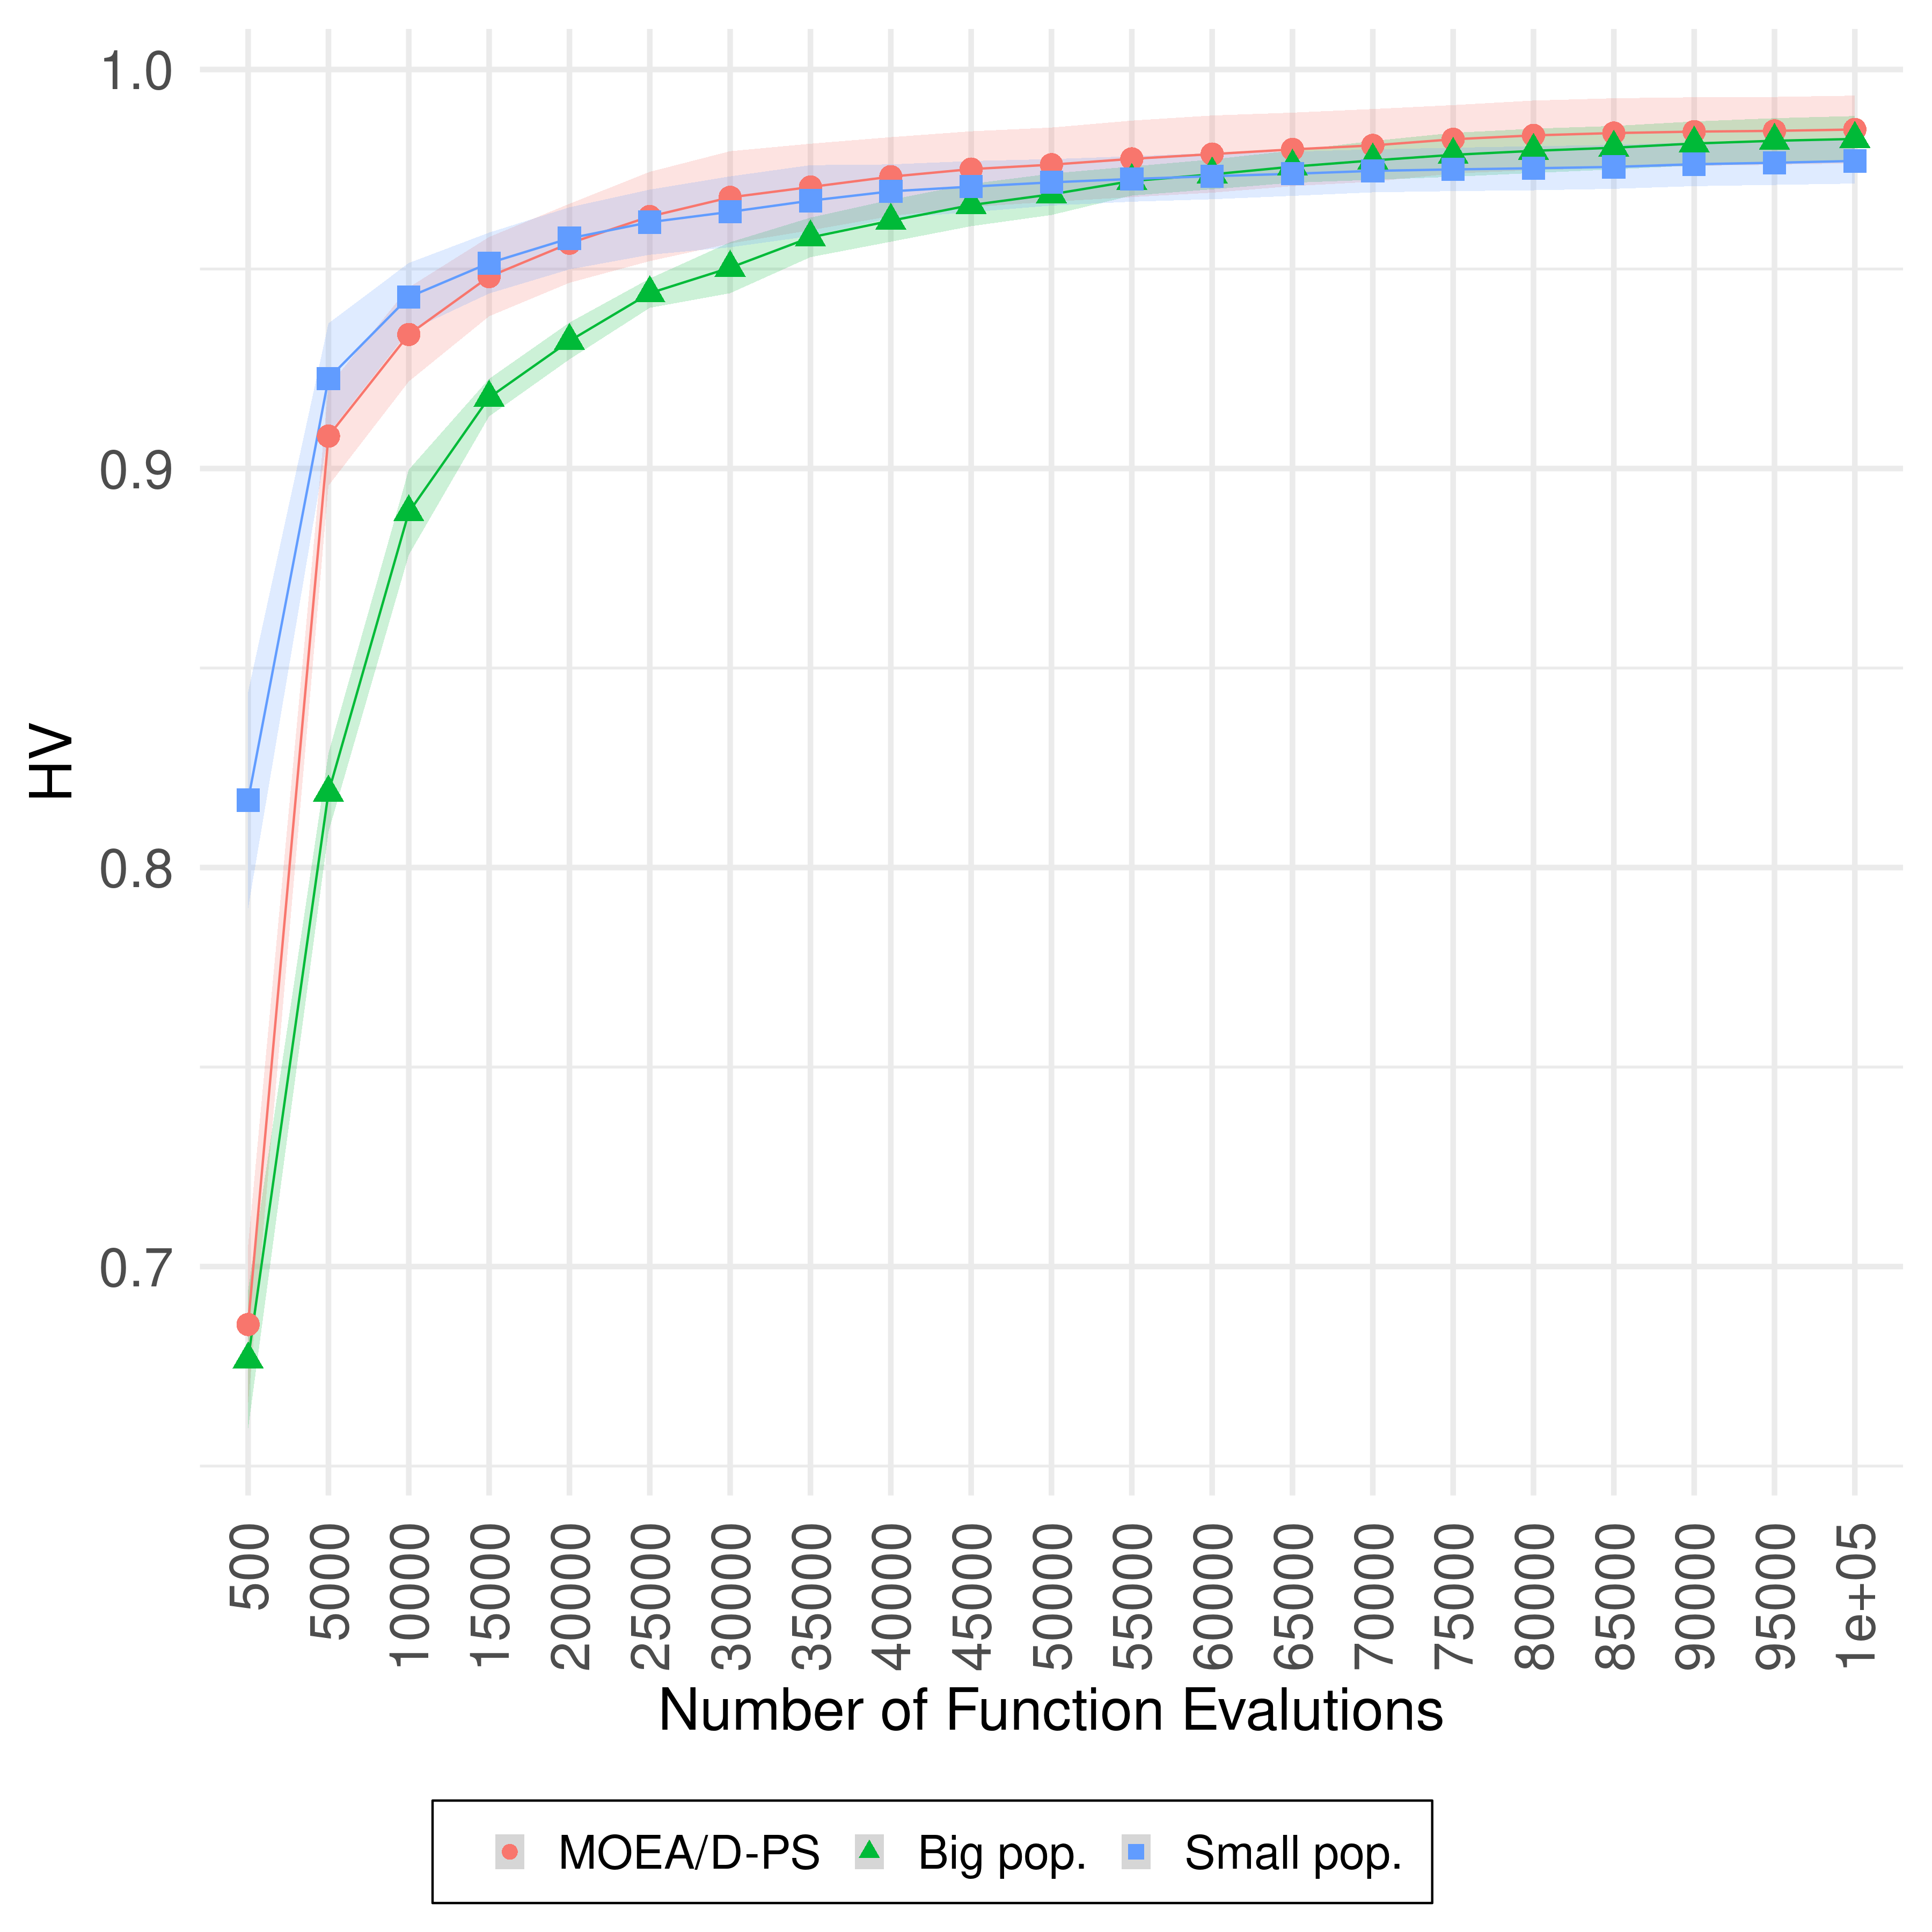
\includegraphics[width=0.45\linewidth]{imgs/UF10hv_evolution}

This image shows the Anytime HV (higher is better, shaded areas indicate
the standard deviation) on UF10. The performance of MOEA/D-PS is shown
as the red circles, MOEA/D with population size 500 is shown as the
green triangles, and MOEA/D with population size equals 50 is shown as
the blue squares, on UF10. The anytime performance of MOEA/D-PS is
similar to the anytime performance of MOEA/D with a small population. We
can see that the three variants have almost the same performance at the
end of the search. This image and text are from {[}5{]}.

See? The 3 algorithms have the same final performance, but how they got
there was different.

\includegraphics[width=0.4\linewidth]{gifs/insightful}

\hypertarget{empirical-attainment-performance}{%
\subparagraph{Empirical Attainment
Performance}\label{empirical-attainment-performance}}

The empirical attainment function (EAF) allows the examination of the
solution many sets of different runs of an algorithm. It can illustrate
where and by how much the outcomes of the two algorithms differ in the
objective space {[}6{]}. The EAF is based on the attainment surface and
resents the probability that an arbitrary objective region in the
objective space is attained (dominated or equal) by an algorithm, and
probability can be estimated using data collected from several
independent runs such algorithm. The attained surface separates the
objective space into two regions: (1) where the objective space is
dominated (attained) by solutions of many sets and (2) where the
objective space is not dominated by those solutions {[}7,8{]}. For
example, the median attainment surface shows regions dominated by at
least half of the runs {[}6{]}.

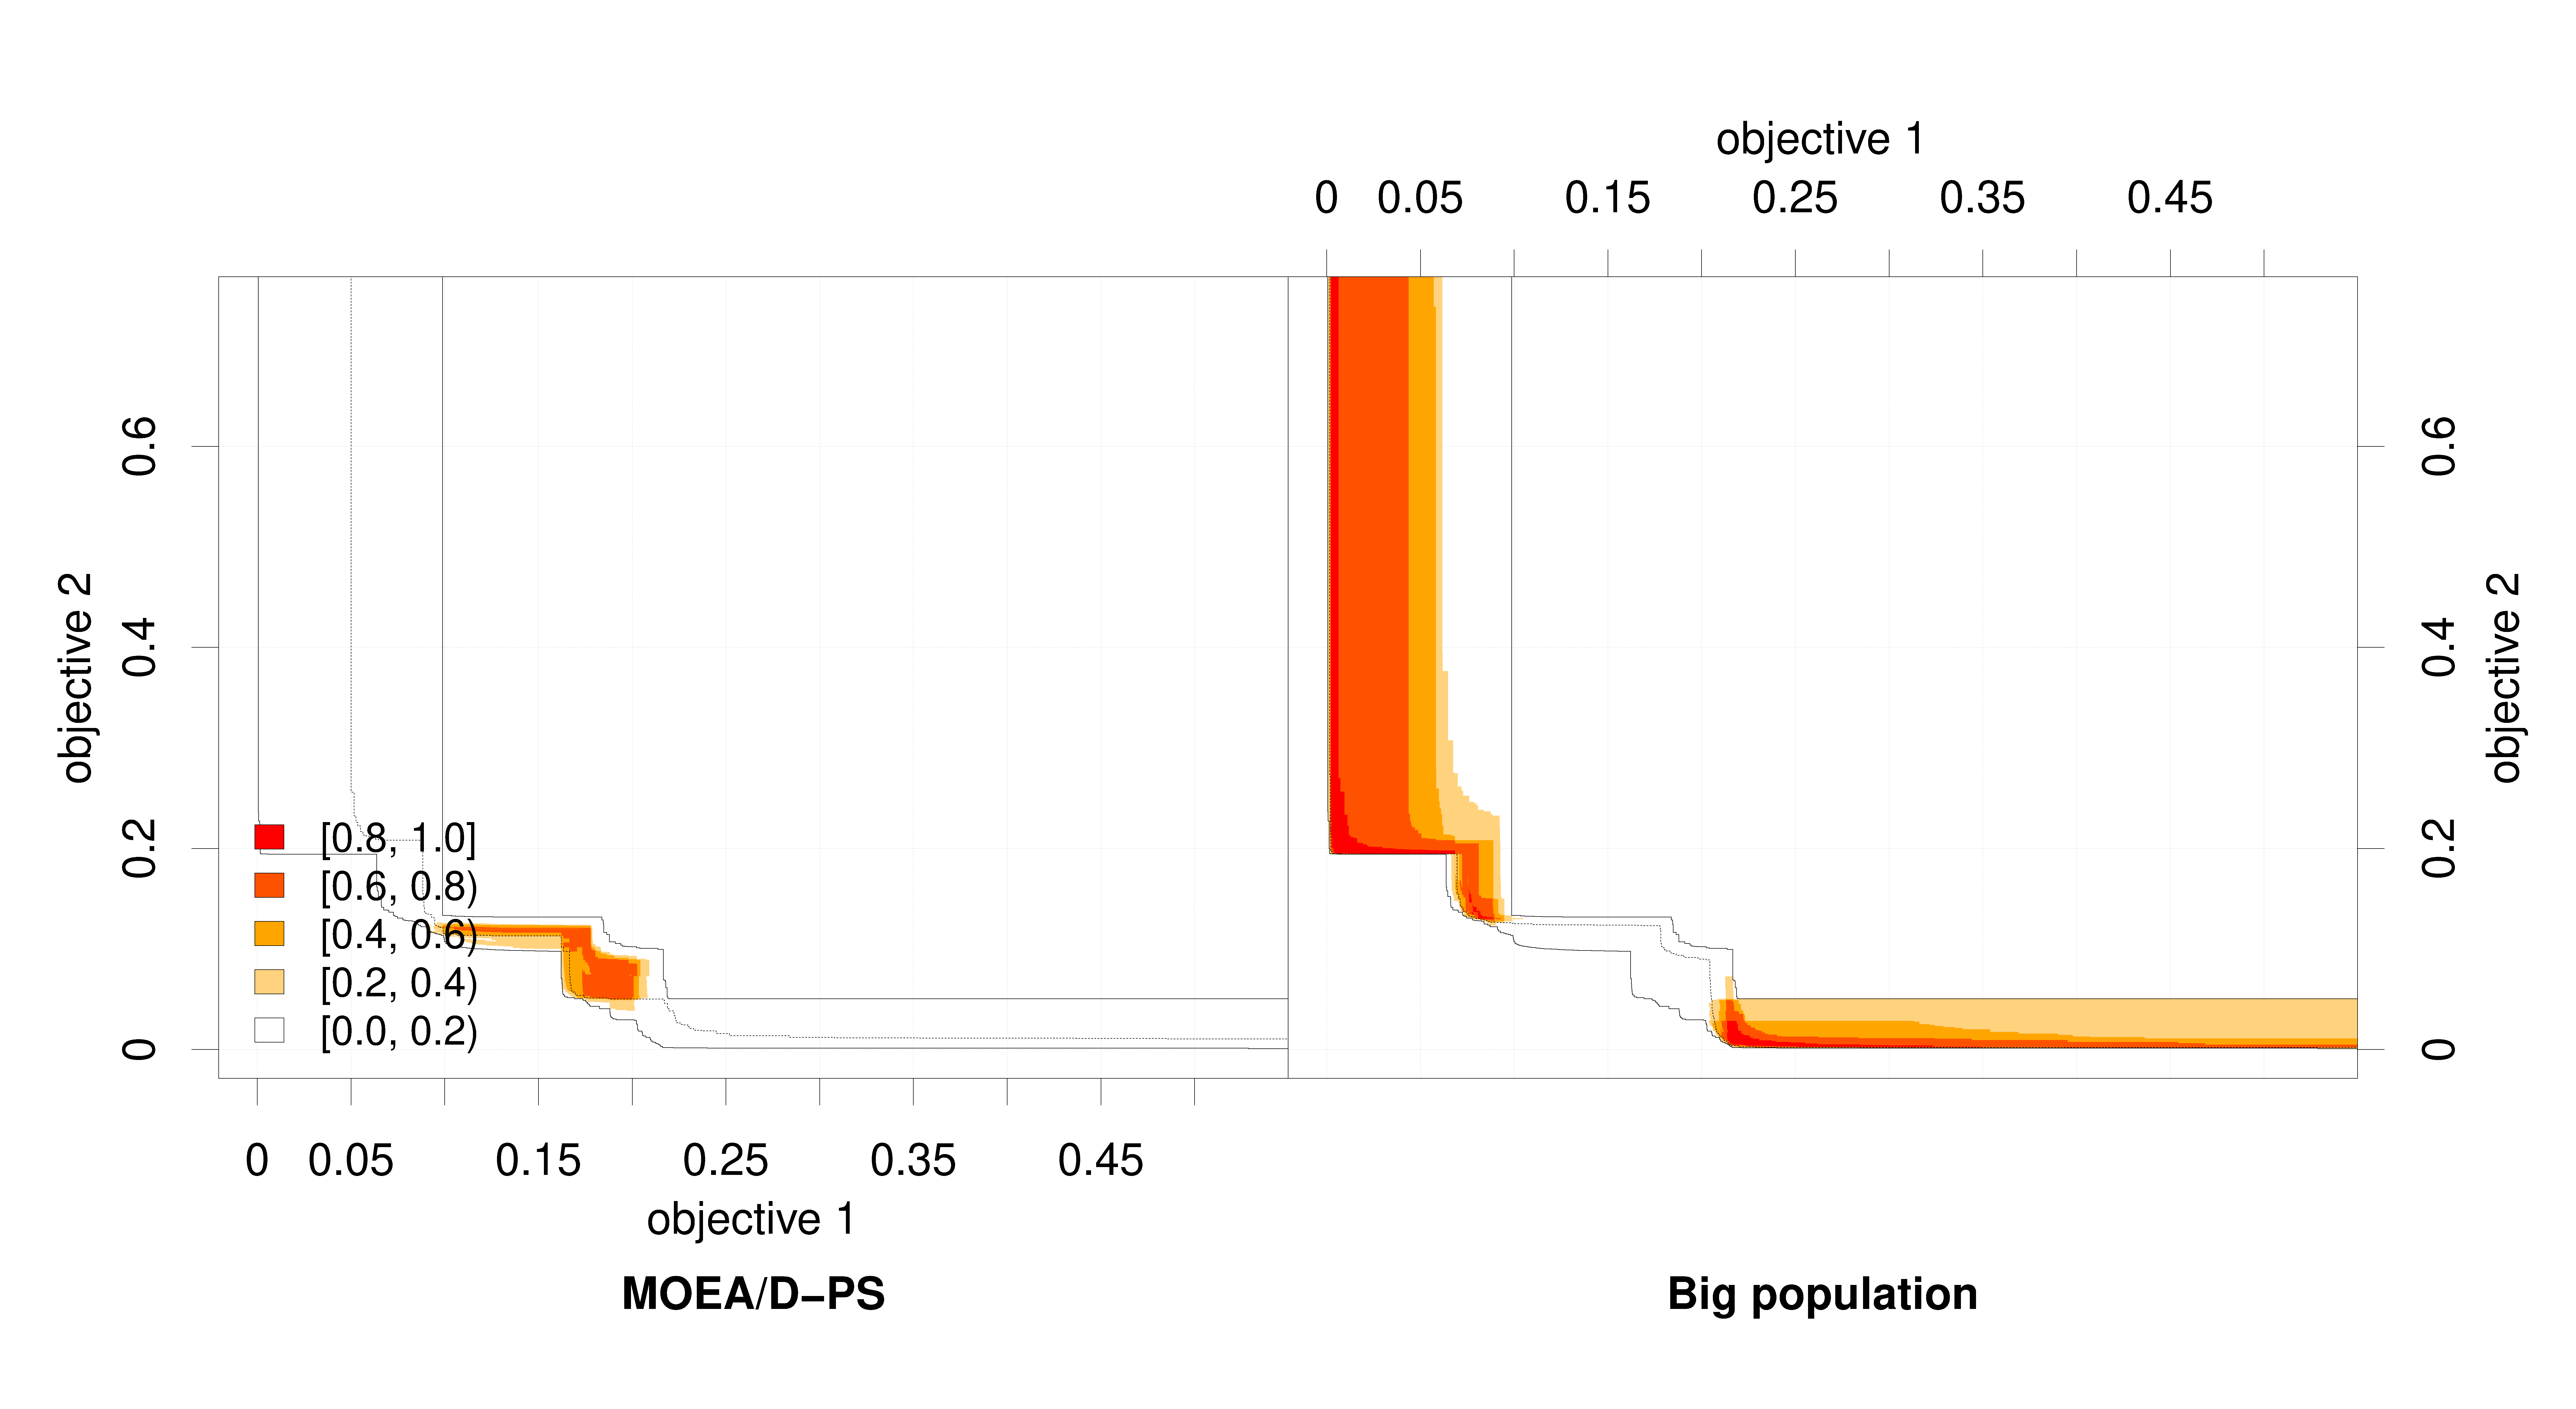
\includegraphics[width=0.65\linewidth]{imgs/eaf_UF6_big_vs_ps}

The shades of red show the amount of the differences of the
probabilistic distribution of the outcomes obtained by the algorithms:
shades closer to red indicate higher differences between the probability
distributions, shades closer to orange indicate little difference and
shades closer to white indicate no difference. Again, this image and
text are from {[}5{]}.

See? The algorithm on the left performs better at central regions of the
objective space. The algorithm on the right performs better at the side
regions. So, if you prefer more balanced solutions, choose the algorithm
from the left, if you prefer extreme solutions, then the one of the
right is the right one.

\includegraphics[width=0.4\linewidth]{gifs/choices}

\hypertarget{search-trajectory-networks}{%
\subparagraph{Search Trajectory
Networks}\label{search-trajectory-networks}}

Search Trajectories Networks (STNs) of multiobjective evolutionary
algorithms is a new tool that I, together with Gabriela Ochoa and Claus
Aranha, have developed and just been accepted for publication at this
year's EvoStar conference.

\includegraphics[width=0.4\linewidth]{gifs/thats_good}

PS: I've been nominated as an ``Outstanding Student'' for this work!

\includegraphics[width=0.4\linewidth]{gifs/cool_peralta}

(Disclaimer: Another meme that I love and that I couldn't resist adding
here. 99!)

In our work, we extend the search trajectory networks models (STNs)
proposed for single objective EAs. The main difference between STNs in
the singleobjective and the multiobjective domains is that we use the
idea of decomposition. The decomposition transforms a multiobjective
problem into several single-objective problems. So, now we can create
STNs for the multiobjective domain!

To see how effective this STN are, we generated STNs models for MOEA/D
and NSGA-II. First, I'm showing the STN of the MOEA/D on the UF10
problem:

\includegraphics[width=0.5\linewidth]{gifs/moead_uf10}

First, I'm showing the STN of the NSGA-II on the same problem:

\includegraphics[width=0.5\linewidth]{gifs/nsga2_uf10}

See how different they are? For example, the first STN, of MOEA/D, is
much more dense that the STN of NSGA-II. Not only that, but the MOEA/D
STN showed more nodes (coloured circles) indicating that the algorithm
is exploring more the search space, while the NSGA-II STN keeps going
back to the end node (the size of the black triangle indicates that this
node is reached multiple times).

Analysing the STNs showed us that we can effectively apply them to
differentiate multiobjective EAs visually and quantitatively. This is
great because we can add together this information to the traditional
comparing metrics, such as HV and IGD.

\includegraphics[width=0.5\linewidth]{gifs/good_job}

Also, they are beautiful! Or is it just me?

For more information, see this Twitter thread.

\url{https://twitter.com/yurilavinas/status/1499681390019092487}

Or read the preprint version: \url{https://t.co/1GAkPy0R9K}.

\begin{center}\rule{0.5\linewidth}{0.5pt}\end{center}

Well, this is it for today. I hope you found this helpful. See you next
time!

\includegraphics{gifs/spongebob-done.gif}

\hypertarget{references}{%
\section{References}\label{references}}

{[}1{]} Zilberstein, S. (1996). Using anytime algorithms in intelligent
systems. AI magazine, 17(3), 73-73.

{[}2{]} Radulescu, A., López-Ibánez, M., \& Stützle, T. (2013, March).
Automatically improving the anytime behaviour of multiobjective
evolutionary algorithms. In International Conference on Evolutionary
Multi-Criterion Optimization (pp.~825-840). Springer, Berlin,
Heidelberg.

{[}3{]} Dubois-Lacoste, J., López-Ibáñez, M., \& Stützle, T. (2015).
Anytime Pareto local search. European journal of operational research,
243(2), 369-385.

{[}4{]} Tanabe, R., Ishibuchi, H., \& Oyama, A. (2017). Benchmarking
multi-and many-objective evolutionary algorithms under two optimisation
scenarios. IEEE Access, 5, 19597-19619.

{[}5{]} Lavinas, Y., Aranha, C., \& Ladeira, M. (2022). Faster
Convergence in Multiobjective Optimisation Algorithms Based on
Decomposition. Evol Comput 2022; DOI:
\url{https://doi.org/10.1162/evco_a_00306}.

{[}6{]} López-Ibáñez, M., Paquete, L., \& Stützle, T. (2010).
Exploratory analysis of stochastic local search algorithms in
biobjective optimisation. In Experimental methods for the analysis of
optimisation algorithms (pp.~209-222). Springer, Berlin, Heidelberg.

{[}7{]} Fonseca, C. M., \& Fleming, P. J. (1996, September). On the
performance assessment and comparison of stochastic multiobjective
optimisers. In International Conference on Parallel Problem Solving from
Nature (pp.~584-593). Springer, Berlin, Heidelberg.

{[}8{]} Fonseca, V. G. D., Fonseca, C. M., \& Hall, A. O. (2001, March).
Inferential performance assessment of stochastic optimisers and the
attainment function. In International Conference on Evolutionary
Multi-Criterion Optimization (pp.~213-225). Springer, Berlin,
Heidelberg.

{[}9{]} Lavinas, Y., Aranha, C., \& Ochoa, G. (2022). Search
Trajectories Networks of Multiobjective Evolutionary Algorithms. arXiv
preprint arXiv:2201.11726.

<!--radix_placeholder_site_after_body-->
<!--/radix_placeholder_site_after_body-->

<!--radix_placeholder_navigation_after_body-->
<div class="distill-site-nav distill-site-footer">

</div>
<!--/radix_placeholder_navigation_after_body-->


\end{document}
